\documentclass{bmcart}

%%%%%%%%%%%%%%%%%%%%%%%%%%%%%%%%%%%%%%%%%%%%%%
%%                                          %%
%% CARGA DE PAQUETES DE LATEX               %%
%%                                          %%
%%%%%%%%%%%%%%%%%%%%%%%%%%%%%%%%%%%%%%%%%%%%%%

%%% Load packages
\usepackage{amsthm,amsmath}
\usepackage{graphicx}
%\RequirePackage[numbers]{natbib}
\RequirePackage{hyperref}
\usepackage[hidelinks]{hyperref}
\usepackage[usenames]{color}
\usepackage[utf8]{inputenc} %unicode support
%\usepackage[applemac]{inputenc} %applemac support if unicode package fails
%\usepackage[latin1]{inputenc} %UNIX support if unicode package fails


%%%%%%%%%%%%%%%%%%%%%%%%%%%%%%%%%%%%%%%%%%%%%%
%%                                          %%
%% COMIENZO DEL DOCUMENTO                   %%
%%                                          %%
%%%%%%%%%%%%%%%%%%%%%%%%%%%%%%%%%%%%%%%%%%%%%%

\begin{document}

	\begin{frontmatter}
	
		\begin{fmbox}
			\dochead{Research}
			
			%%%%%%%%%%%%%%%%%%%%%%%%%%%%%%%%%%%%%%%%%%%%%%
			%% INTRODUCIR TITULO PROYECTO               %%
			%%%%%%%%%%%%%%%%%%%%%%%%%%%%%%%%%%%%%%%%%%%%%%
			
			\title{Comorbilidades COVID-19}
			
			%%%%%%%%%%%%%%%%%%%%%%%%%%%%%%%%%%%%%%%%%%%%%%
			%% AUTORES. METER UNA ENTRADA AUTHOR        %%
			%% POR PERSONA                              %%
			%%%%%%%%%%%%%%%%%%%%%%%%%%%%%%%%%%%%%%%%%%%%%%
			
			\author[
			  addressref={aff1},                   % ESTA LINEA SE COPIA IGUAL PARA CADA AUTOR
			  corref={aff1},                       % ESTA LINEA SOLO DEBE TENERLA EL COORDINADOR DEL GRUPO
			  email={inesdiazdelrey@gmail.com}   % VUESTRO CORREO ACTIVO
			]{\inits{I.D.R.}\fnm{Inés} \snm{Díaz del Rey}} % inits: INICIALES DE AUTOR, fnm: NOMBRE DE AUTOR, snm: APELLIDOS DE AUTOR
			\author[
			  addressref={aff1},
			  email={rythemond@gmail.com}
			]{\inits{M.L.P.R.}\fnm{Miguel Leonardo} \snm{Padilla Romo}}
			\author[
			addressref={aff1},
			email={claauudiiaa24@gmail.com}
			]{\inits{C.V.R.}\fnm{Claudia} \snm{Vega Rodríguez}}
			
			%%%%%%%%%%%%%%%%%%%%%%%%%%%%%%%%%%%%%%%%%%%%%%
			%% AFILIACION. NO TOCAR                     %%
			%%%%%%%%%%%%%%%%%%%%%%%%%%%%%%%%%%%%%%%%%%%%%%
			
			\address[id=aff1]{%                           % unique id
			  \orgdiv{ETSI Informática},             % department, if any
			  \orgname{Universidad de Málaga},          % university, etc
			  \city{Málaga},                              % city
			  \cny{España}                                    % country
			}
		
		\end{fmbox}% comment this for two column layout
		
		\begin{abstractbox}
		
			\begin{abstract} 
			

			Debido a la nueva normalidad provocada por la COVID-19 durante estos últimos dos años, los estudios relacionados con esta enfermedad han traído información esclarecedora en cuanto a su funcionamiento. En este caso, deseamos ver las morbilidades que se asocian con la Covid-19. Esto ayudará a identificar qué otros trastornos y patologías favorecerían su desarrollo o debilitarían al individuo frente a un posible contagio.

			\newline

			Se ha recolectado información sobre la red PPI de la COVID-19 y obtenido todas las proteínas relevantes. A partir de varias búsquedas en \textit{PheGenI}, se consigue más información sobre las otras patologías a las que estas mismas proteínas están asociadas y se obtienen para componer los diferentes nodos de la red de comorbilidades que se generarán luego. Se realiza un preprocesamiento previo pues, aunque las proteínas están relacionadas con el organismo humano, no todas  tienen una enfermedad relevante asociada. Con esto, se reduce el tamaño de la red y la se mantiene coherente.

			\newline

			Diseñando programas en \textit{R}, se ejecuta el código necesario para construir los modelos de redes y analizar las comorbilidades de COVID-19. Se observa que hay algunas patologías que interaccionan más fuertemente e indican mayor susceptibilidad a contraer la enfermedad, tales como el cáncer, la enfermedad de Parkinson o el Alzheimer.

			%%%%%%%%%%%%%%%%%%%%%%%%%%%%%%%%%%%%%%%%%%%%%%%
			%% RESUMEN BREVE DE NO MAS DE 100 PALABRAS   %%
			%%%%%%%%%%%%%%%%%%%%%%%%%%%%%%%%%%%%%%%%%%%%%%%	
			
			\end{abstract}
			
			%%%%%%%%%%%%%%%%%%%%%%%%%%%%%%%%%%%%%%%%%%%%%%
			%% PALABRAS CLAVE DEL PROYECTO              %%
			%%%%%%%%%%%%%%%%%%%%%%%%%%%%%%%%%%%%%%%%%%%%%%
			
			\begin{keyword}
			\kwd{comorbilidades}
			\kwd{COVID-19}
			\kwd{proteínas}
			\kwd{genes}
			\kwd{enfermedades}
			\kwd{redes}
			\kwd{interacciones}
			\end{keyword}
		
		
		\end{abstractbox}
	
	\end{frontmatter}		
		
	
	%%%%%%%%%%%%%%%%%%%%%%%%%%%%%%%%%
	%% COMIENZO DEL DOCUMENTO REAL %%
	%%%%%%%%%%%%%%%%%%%%%%%%%%%%%%%%%
	
	\section{Introducción}

La \textit{comorbilidad}, también conocida como \textit{morbilidad asociada}, es un término utilizado para describir dos o más trastornos o enfermedades que padece una misma persona. Pueden ocurrir simultánea o secuencialmente. La comorbilidad también implica que existe una interacción entre los dos trastornos, lo que podría empeorar la evolución de ambos.

\newline

En las poblaciones envejecidas del siglo actual, se da la situación de que muchas personas padezcan más de una enfermedad a la vez, lo que se ha convertido en uno de los principales retos a solucionar, pues, al afectar principalmente a esta población, se disminuyen las opciones de tratamiento y esperanza de vida de los pacientes. En los estudios realizados a erca de las relaciones de comorbilidad, se proporciona una visión global de la probabilidad, ya sea mayor o menor, de desarrollar enfermedades secundarias asociadas a una enfermedad previa.

\newline

De este modo, se ha podido observar que la población anciana es más susceptible a la enfermedad COVID-19 y, además, tiene una mayor probabilidad de ser ingresada en la UCI con una mayor tasa de mortalidad. 
Debido a que la COVID-19 es una enfermedad relativamente nueva, los datos de estudio disponibles son limitados. Sin embargo, se ha podido observar que las comorbilidades aumentan las posibilidades de contraer la enfermedad. En este artículo, se tratará acerca de las comorbilidades de la COVID-19.

\newline

En primer lugar, se obtuvieron las proteínas virales del SARS-CoV2 de las cuáles se recopilaron los genes de las interacciones asociadas. El objetivo principal era obtener las enfermedades vinculadas a las proteínas humanas que interaccionan con las virales, por lo que se realizaron diversas búsquedas en \textit{PheGenI} de los genes asociados para comprobar si tenían alguna enfermedad asociada o no. Todos los genes estaban relacionados con diferentes procesos en el organismo humano, pero no fueron tantos los vinculados a enfermedades.

\newline

A lo largo de este artículo, se desarrollarán los procedimientos tomados para determinar las comorbilidades de la COVID-19, es decir, para concretar cuáles son las enfermedades que provocan en las personas que las padecen más susceptibilidad a contraer la infección por SARS-CoV2.

	\section{Materiales y métodos}

\subsection{Obtención de proteínas y genes asociados}

El primer paso fue obtener las proteínas virales del SARS-CoV2, para ello se recurrió a \textit{STRING}, una base de datos de interacciones proteína-proteína. Concretamente, se accedió a una \href{https://string-db.org/cgi/covid.pl}{\textcolor{Cyan}{\underline{página de STRING}}} donde se recopilan las proteínas asociadas al virus y sus interacciones. A partir de ella, se fue seleccionando cada proteína viral con el fin de observar cuáles eran los genes que estaban asociados a cada una y guardarlos en archivos \textit{.tsv}. Las proteínas que se asociaron al SARS-CoV2 son \textit{E, M, N, Spike, nsp1, nsp2, nsp3, nsp4, nsp5, nsp6, nsp7, nsp8, nsp9, nsp10, nsp11, nsp12, nsp13, nsp14, nsp15, orf3a, orf3b, orf6, orf7a, orf8, orf9b, orf9c, orf10}. En los ficheros de formato \textit{TSV}, se almacenan las interacciones entre los genes de cada proteína con separaciones de tabulares entre cada columna. En las columnas, se asocian los nombres \textit{node1} y \textit{node2} para los genes que interaccionan y, el resto se denominan \textit{node1 accession}, \textit{node2 accession}, \textit{node1 annotation}, \textit{node2 annotation} y \textit{score}. 

\newline

Una vez recopilados los ficheros de formato \textit{TSV}, se guardaron en el proyecto para, posteriormente, poder ser utilizados en el desarrollo del código en \textit{R}. Se comentará en más detalle en la sección \textit{Generación de análisis de red PPI}.

\subsection{Búsqueda de enfermedades relacionadas}

Una vez recopiladas las interacciones de los genes asociados a las proteínas, se extrajeron el nombre de aquellos genes involucrados en dichas interacciones. El total de estos genes fue de 246, por lo que se tuvo que realizar una búsqueda de todos ellos con el fin de recopilar información a cerca de posibles enfermedades que pudieran estar relacionadas con los seres humanos. Dicha búsqueda se hizo por medio del integrador \href{https://www.ncbi.nlm.nih.gov/gap/phegeni}{\textcolor{Cyan}{\underline{Phenotype-Genotype Integrator (PheGenI)}}, el cual se fusiona con varias bases de datos alojadas en el Centro Nacional de Biotecnología Información (NCBI). 
	
\newline
	
Finalmente, se obtuvieron enfermedades relacionadas para 75 genes. Para los 171 genes restantes no se encontró ninguna enfermedad asociada a ellos. Entre las enfermedades encontramos gran diversidad como diferentes tipos de cáncer, síndromes, Parkinson, Alzheimer, entre otras. Se comentará en más detalle en la sección \textit{Resultados}.

\subsection{Generación de análisis de red PPI}

En esta sección, se comentará el desarrollo realizado en el lenguaje R. Las librerías que se usaron son \textit{STRINGdb}, \textit{igraph} y \textit{linkcomm}. El paquete \textit{STRINGdb} proporciona una interfaz R para la base de datos de interacciones proteína-proteína \href{http://www.string-db.org}{\textcolor{Cyan}{\underline{STRING}}. El paquete \textit{igraph} recopila una colección de herramientas de análisis de redes con énfasis en la portabilidad, eficiencia y facilidad de uso del código. El paquete \textit{linkcomm} proporciona herramientas para generar, visualizar y analizar \textit{Link Communities} en redes. Tanto el paquete \textit{igraph} como el paquete \textit{linkcomm} se encuentran en \textit{CRAN}, en cambio, el paquete \textit{STRINGdb} se debe instalar por medio de \textit{BioConductor}.
	
\newline
	
Tras llamar a las librerías necesarias, se cargaron todos los archivos \textit{.tsv} descargados de \textit{STRING} que recopilan las interacciones de los genes para cada proteína viral. Y a su vez, se agregaron todas las variables en las que se cargaron estos archivos en una única variable. A partir de ella, gracias al paquete \textit{STRINGdb}, se creó un nuevo objeto \textit{STRING\_db} asociado a la especie \textit{Homo Sapiens}, para poder observar las interacciones de los genes recopilados para el ser humano. Se realizó un mapeo de los genes y se generó la red de interacción de los genes de las proteínas. 

\newline

El siguiente paso fue guardar la recopilación de genes y enfermedades en una nueva variable, con el fin de poder observar la relación entre ellos. Para poder obtener resultados más óptimos, únicamente se consideraron aquellos genes que tuvieran enfermedades asociadas. Primero, se intentó representar una red con los genes y enfermedades por medio del paquete \textit{igraph}, al observar que no era el mejor método debido a la representación que se obtuvo, se decidió realizarla por medio del paquete \textit{linkcomm}. De este modo, se podría mostrar las comunidades existentes en la red de los genes y enfermedades asociadas.

\newline

Para una mejor visualización de lo comentado en esta parte, se detallará en la sección \textit{Resultados}.

	\section{Resultados}

En esta sección, se comentarán los resultados obtenidos tras la investigación realizada. Dicha investigación ha tomado los siguientes pasos: búsqueda de proteínas virales del SARS-CoV2 y genes asociados a ellas, búsqueda de las enfermedades relacionadas con los genes de las proteínas y desarrollo de código para el análisis de red PPI.

\newline

Para la primera parte de la ejecución se cargaron los datos recopilados en \textit{STRING}, es decir, los genes asociados a las proteínas virales del virus. Tras agrupar todos los datos, se creó un objeto de \textit{STRINGdb}, se mapeó y se generó la red de interacción. A continuación, podemos observar la siguiente red obtenida.

\newline

\begin{figure}[h!]
	\includegraphics[width=0.9\textwidth]{../../results/figuraSTRINGdb.png}
	\caption{Interacciones entre genes obtenida por medio de STRINGdb}
	\label{fig:red_stringdb}
\end{figure}

\newline

En dicha figura se muestra una representación de los genes recopilados interaccionando entre ellos pero en la especie \textit{Homo Sapiens}. Se puede observar que en esta especie hay 67 interacciones entre los 246 genes considerados, por lo cual existen bastantes genes que no interaccionan entre ellos.

\newline

Para la segunda parte de la ejecución del código era necesario realizar la búsqueda de enfermedades asociadas a los diferentes genes por medio de \textit{PheGenI} y guardar estas relaciones en una determinada variable para su uso. Se obtuvo 75 genes con enfermedades asociadas, y para este conjunto se ploteó una red de interacción entre genes y enfermedades por medio de \textit{igraph}. La red obtenida se muestra a continuación.

\newline

\begin{figure}[h!]
	\includegraphics[width=0.9\textwidth]{../../results/figuraiGraph.png}
	\caption{Interacciones genes y enfermedades obtenida por medio de igraph}
	\label{fig:red_igraph}
\end{figure}

\newline

Debido a que no se observaba una clara diferencia entre los nodos, se decidió hacer uso de la librería \textit{linkcomm}.

\newline

Para la tercera y última parte de la ejecución, se generó una red de interacción entre genes y enfermedades en la que se mostrase las comunidades existentes en dicha red. La red creada corresponde con la mostrada a continuación.

\newline

\begin{figure}[h!]
	\includegraphics[width=0.9\textwidth]{../../results/figuraLinkcomm.png}
	\caption{Interacciones genes y enfermedades obtenida por medio de LinkComm}
	\label{fig:red_linkcomm}
\end{figure}

\newline

Se puede observar que gran parte de las enfermedades están asociadas a un solo gen, pero existen algunas que tienen varios genes asociados. 

\newline

Durante la búsqueda de enfermedades relacionadas, se pudo observar que enfermedades como el cáncer, la enfermedad de Parkinson, el Alzheimer o el carcinoma, están relacionadas con varios genes. Esto quiere decir que el individuo con dichas enfermedades será más susceptible a contagiase por COVID-19. Por otro lado, con el resto de enfermedades asociadas ocurrirá lo mismo, aunque las nombradas previamente están asociadas a más de las proteínas estudiadas en esta investigación.

\newline

A modo de interés, las enfermedades que se obtuvieron tras la búsqueda y que por lo tanto, están relacionadas con la susceptibilidad de contraer la enfermedad COVID-19, son \textit{juvenile myoclonic epilepsy, upper respiratory tract carcinoma, familial hyperlysinemia, medium-chain acyl-CoA dehydrogenase deficiency, type II glutaricaciduria, alzheimer's disease, autosomal recessive spinocerebellar ataxia-2, retinitis pigmentosa, hereditary stomatocytosis, hypertension, ANE syndrome, parkinson's disease, cancer, juvenile myelomonocytic leukemia, serous endometrial tumors, hereditary sensory neuropathy type IE, carcinoma, methemoglobinemias, type IIb congenital disorder of glycosylation, warburg micro syndrome type 3, charcot-marie-tooth (CMT) type 2 neuropathy, hiatt-neu-cooper syndrome, gastric cancer, hashimoto's thyroiditis, pediatric acute myeloid leukemia, SHRF disease, pontocerebellar hypoplasia, alazami syndrome, sensorineural hearing loss+hypoglycemia, leigh syndrome, kearns-sayre syndrome, alpers' syndrome, severe congenital neutropenia 8, familial bone marrow failure, williams syndrome, age-related macular degeneration type 3, marfan syndrome, congenital contractural arachnodactyly, acute myeloid leukemia, troyer syndrome, complex cortical dysplasia with other brain malformations-5, asymmetric polymicrogyria, hypomyelinating leukodystrophy-6, leber congenital amaurosis, autosomal recessive primary microcephaly-8, schizophrenia, stem cell myeloproliferative disorder, microcephalic osteodysplastic primordial,  dwarfism type II, myeloproliferative disorder, corticotropin-independent Cushing's syndrome, smith-magenis syndrome, leukemia, cancer cachexia, bethlem myopathy, urbach-wiethe disease, tissue hypoxia, tumor invasiveness, thoracic aortic aneurysms, tumor progression, bruck syndrome, marinesco-sjogren syndrome, breast cancers, torsion dystonia 1, acyl-CoA dehydrogenase family member type 9 deficiency, mitochondrial complex III deficiency, mitochondrial complex I deficiency, lethal neonatal disease}.
	\section{Discusión}

Una vez que se han conseguido los resultados correspondientes, se procede a discutir los diferentes problemas y hallazgos en esta sección

\subsection{Análisis inicial de genes y proteínas}

\subsubsection{Red PPI SARS-Cov2}

La red de interacción entre proteínas del SARS-Cov2 se compone de un total de \emph{332 proteínas cebo del virus que interactúan con el organismo humano}. Una proteína cebo es aquella que se usa para identificar las interacciones de las otras proteínas que nos interesa analizar (conocidas como \textit{proteínas cebo}). Suelen ser elegidas aquellas de las que se dispone información 

\newline

La red mostrada a continuación muestra un esquema de colores que identifican aquellas proteínas que participan en una misma interacción viral. En la figura se muestran las 10 proteínas con mayor interacción entre ellas así como otras 15 adicionales que, según Uniprot, son relevantes para la enfermedad. Tenemos un total de \emph{25 proteínas} que forman un total de \emph{61 interacciones} a nivel global de red con una media aproximada de \emph{grado de 4.88}.El \textit{p} valor es prácticamente nulo \textit{(0.000173}:

	\begin{figure}[h!]
		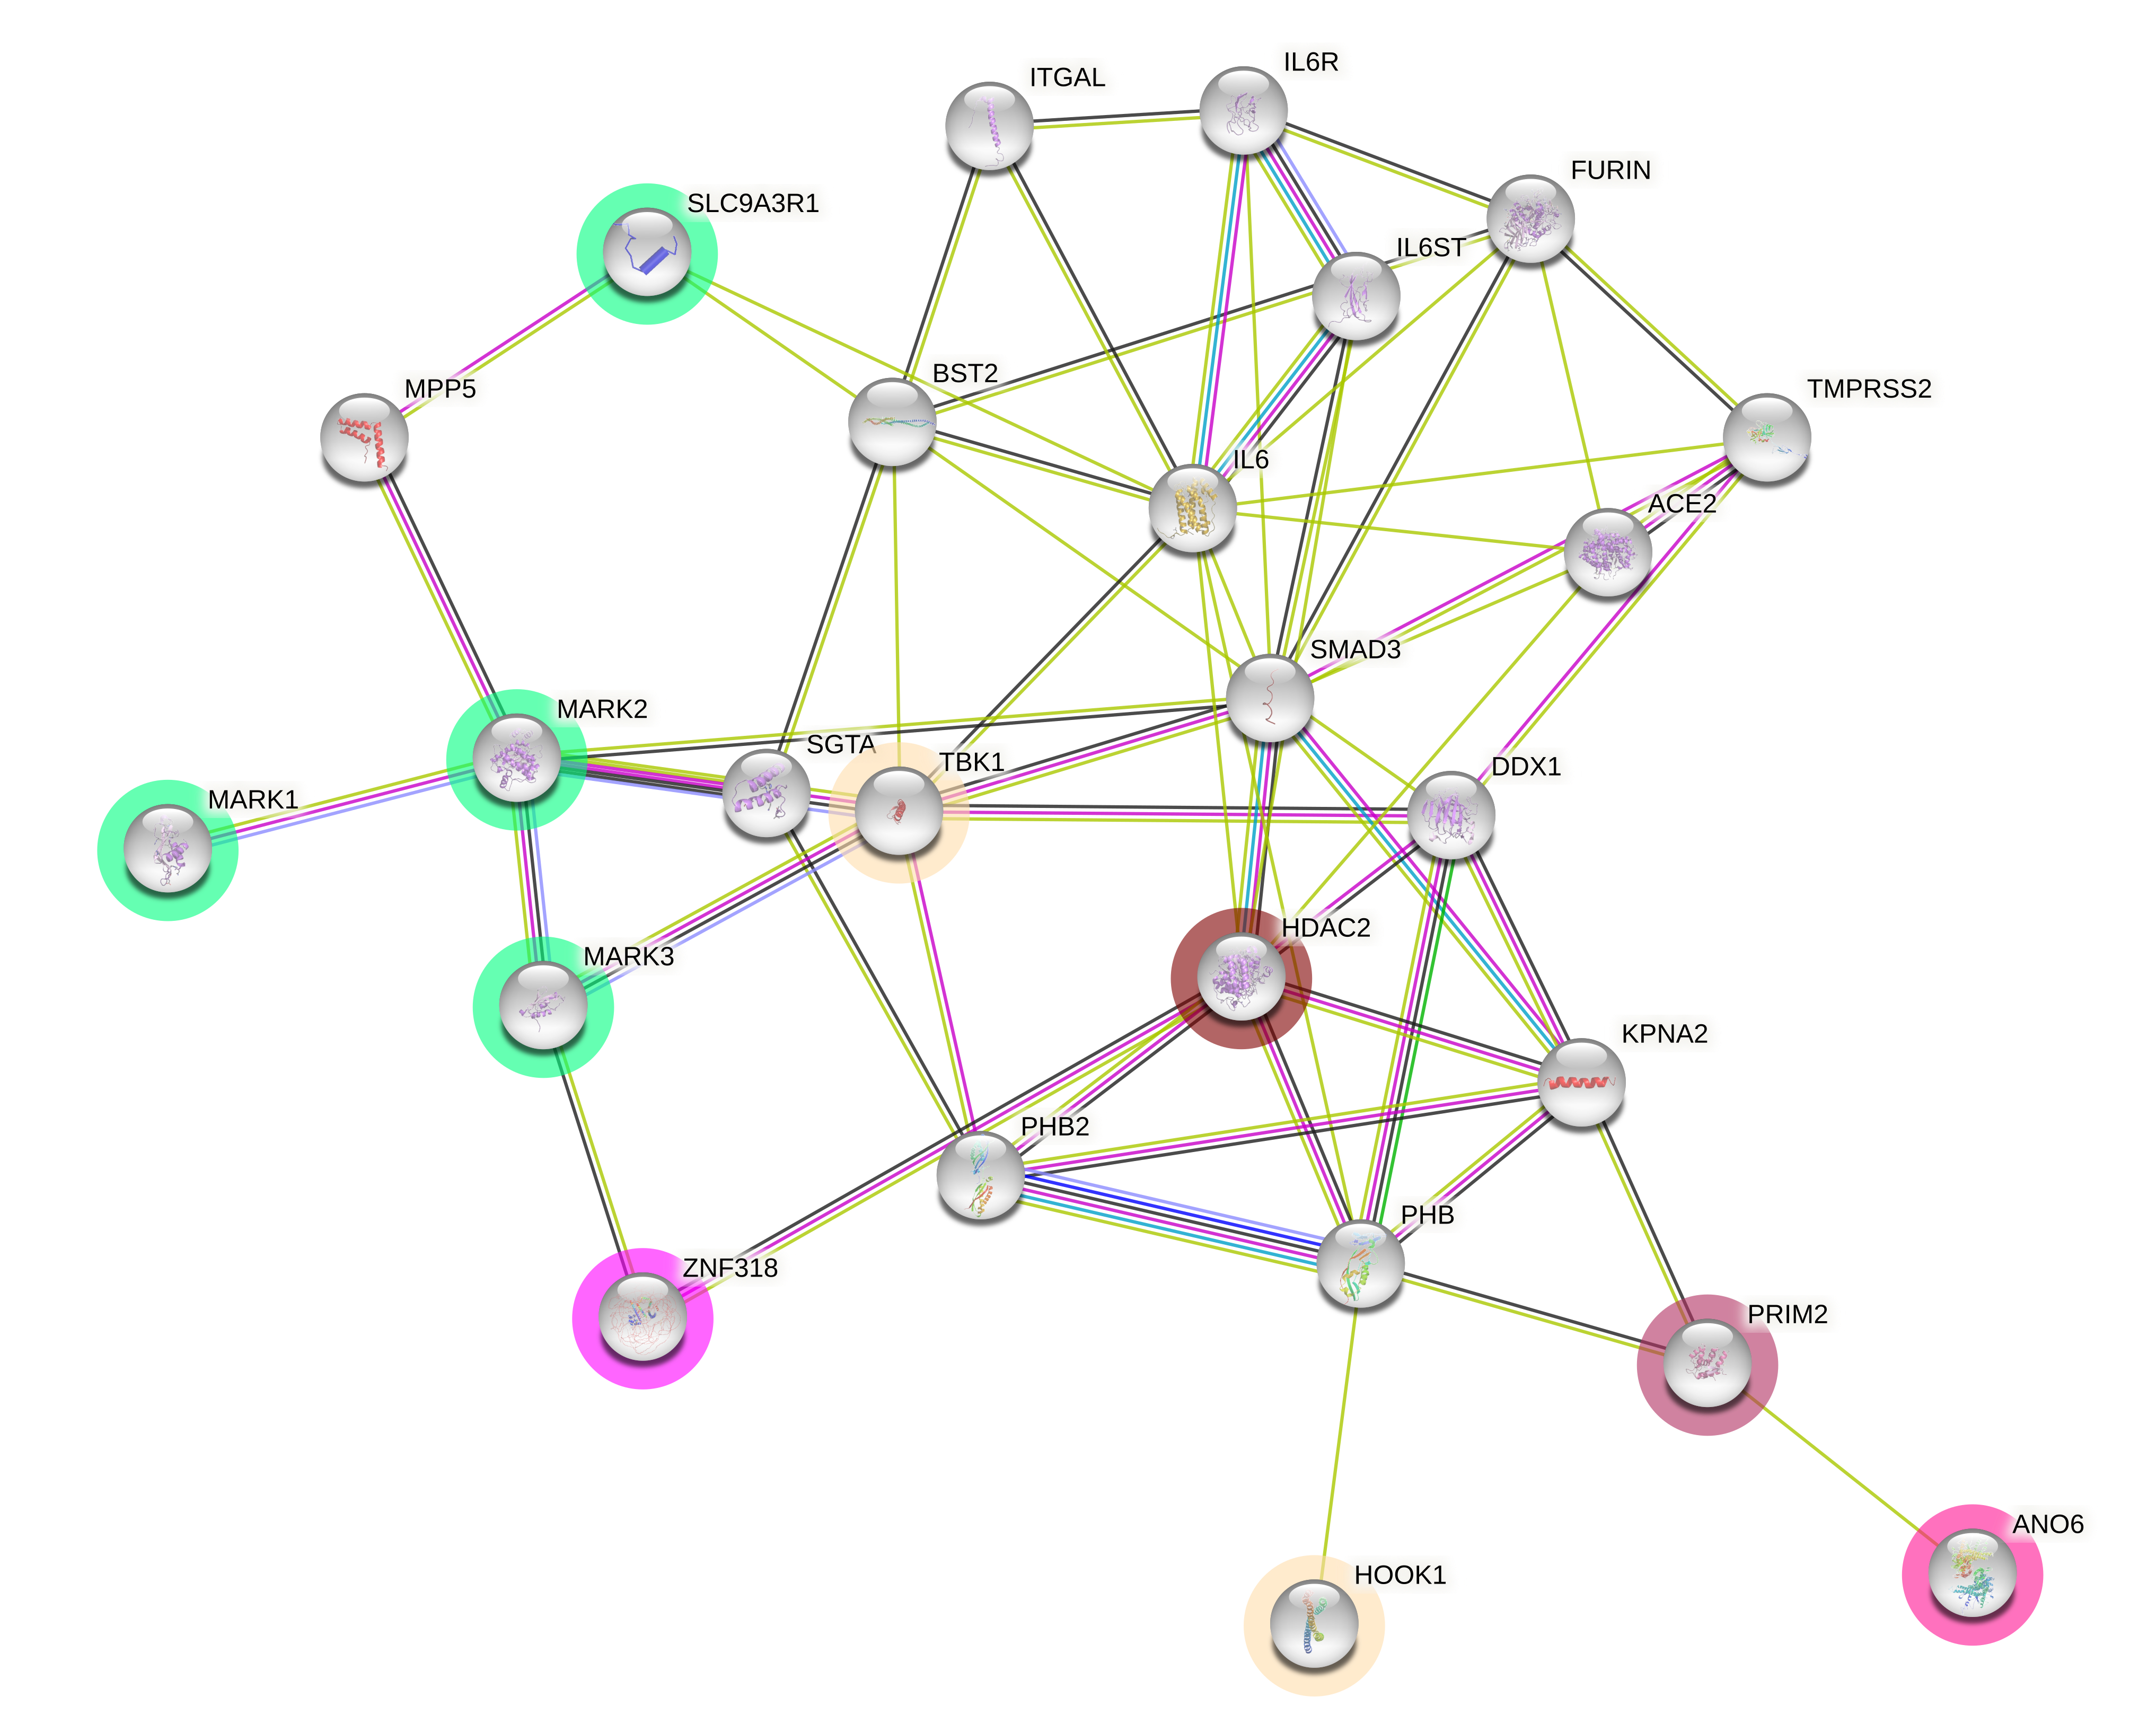
\includegraphics[width=0.9\textwidth]{figures/PPInetSARSCov2BaitProt.png}
		\caption{SARS-CoV-2 protein interaction map}
		\label{fig:ppi_net}
	\end{figure}
	
	\begin{figure}[h!]
		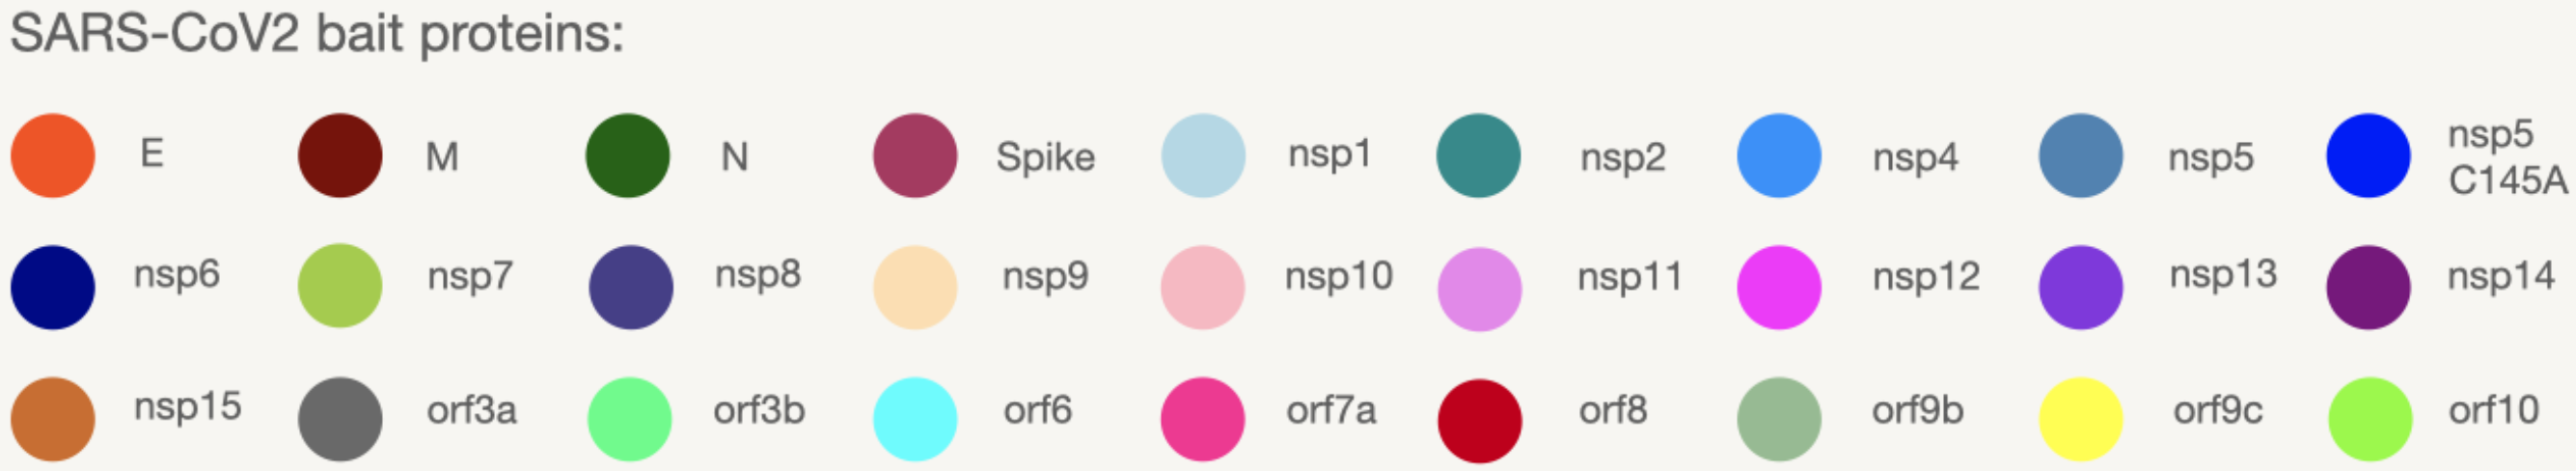
\includegraphics[width=0.9\textwidth]{figures/PPIColourLegend.png}
		\caption{Colour Legend}
		\label{fig:ppi_legend}
	\end{figure}

Se procede a descargar la información casi completa de toda la red (246 de las 332 proteínas) en forma de archivos \textit{tsv} para su posterior lectura y graficación usando código en \textit{R}. Se observa que, del total, tan sólo \emph{existen interacciones significativas entre 67 proteínas cuando originalmente se esperaban 4 interacciones} a nivel global de la red. El elevado número de interacciones nos indica que esta red no es fruto del azar(como prueba el \textit{p} valor de 0), si no que se trata de un red real e indicativo de que las proteínas probablemente están asociadas a funciones biológicas.

	\begin{figure}[h!]
		\includegraphics[width=0.9\textwidth]{figures/figuraSTRINGdb.png}
		\caption{Full protein interaction map}
		\label{fig:ppi_stringdb}
	\end{figure}

Ahora se tiene la absoluta certeza de que estas proteínas pueden estar asociadas entre sí y, por lo tanto, posiblemente puedan estar relacionadas con otras patologías a través de sus fenotipos.
	
\subsection{Análisis de comorbilidades}

Usando los datos recopilados en el archivo \textit{nodes&diseases.tsv} en el que se encuentran asociadas las proteínas y sus posibles enfermedades derivadas, se puede visualizar el subconjunto de aquellas que filas que contenga una proteína y su enfermedad (se desechan aquellas con las que no se tenga información de su patología correspondiente). La red resultante de \textit{iGraph} de 75 nodos queda de la siguiente forma:

	\begin{figure}[h!]
		\includegraphics[width=0.9\textwidth]{figures/figuraiGraph.png}
		\caption{Partial protein-disease network (iGraph)}
		\label{fig:ppi_sigraph}
	\end{figure}
	
Aunque algo desordenada, se puede apreciar que hay enfermedades que hay nodos de tipo \textit{proteína} y nodos del tipo \textit{enfermedad} (sin diferencias visuales aparentes). Aquellos nodos que se encuentren más cercanos entre sí guardan una relación y viceversa. Se decide probar una nueva y mejor representación usando el paquete \texit{R} de \texit{linkcomm}. Se encuentran nodos más grandes que otros, indicativo de un grado superior y su mayor nivel de conectividad. Estos nodos coinciden con proteínas, con lo que se deduce que \emph{una importante minoría de proteínas están relacionadas con más de una patología} u otra proteína con su patología correspondiente. Podemos destacar \texit{COL6A1,  ACLADM y la PMCA }, aunque también se ve una enfermedad que está asociada a varias proteínas.

	\begin{figure}[h!]
		\includegraphics[width=0.9\textwidth]{figures/figuraLinkcomm.png}
		\caption{Partial protein-disease network (linkcomm)}
		\label{fig:ppi_linkcomm}
	\end{figure}
	
Tal como se puede ver, \emph{se ha logrado un mapa con cierto nivel de detalle sobre las diferentes comorbilidades del SARS-Cov2} usando diferentes paquetes de modelado de redes con \textit{R (stringdb, iGraph, linkcomm}. Se han podido analizar las redes, confirmando las interacciones entre proteínas así como las relaciones que existen con diferentes patologías.
	\section{Conclusiones}

Una de las principales dificultades ha sido encontrar el Dataset de interés para adquirir los genes asociados a la lista de proteínas del SARS-CoV2 poder realizar el correspondiente estudio de las relaciones genes-enfermedades. Esto se solucionó realizando una búsqueda exhaustiva y dando con el resultado de una lista de proteínas del SARS-CoV2 que tenían asociados ciertos genes. 

\newline

A la hora de visualizar las redes de interacciones creadas, la red creada con la librería de iGraph, es decir, la correspondiente a la relación genes-enfermades, se muestra de una forma poco visible ya que nos encontramos con que cada gen poseía única y exclusivamente una enfermedad. 

\newline

Por otro lado, de la red correspondiente a STRINGdb donde se muestra las relaciones de proteínas se puede deducir que se produce una disminución del número de asociaciones ya que se parte de interacciones entre los genes del virus, entonces al asociarse con el genoma humano, la interacción de genes-proteínas cambia porque el resto de genes van asociadas a un genoma distinto. 

\newline

Para concluir, se afirma que se aclararon un poco los resultados cuando se usó Linkcomm, ya que se puede visualizar con casi total claridad el gen que está asociado a cada enfermedad. Por otro lado, no se ha podido obtener el Link Communities y Community centrality debido a que se necesitaba una red mayor para que se consiguiera realizar la agrupación (clusters) convenientes. 

 

 
	
	
	%%%%%%%%%%%%%%%%%%%%%%%%%%%%%%%%%%%%%%%%%%%%%%
	%% OTRA INFORMACIÓN                         %%
	%%%%%%%%%%%%%%%%%%%%%%%%%%%%%%%%%%%%%%%%%%%%%%
	
	\begin{backmatter}
	
		\section*{Abreviaciones}%% if any
			
			PPI: Protein-Protein Interactions
		
		\section*{Disponibilidad de datos y materiales}%% if any
			
			\href{https://github.com/Ines-Diaz/project_template}{\textcolor{Cyan}{\underline{Repositorio GitHub}}}
		
		\section*{Contribución de los autores}
			
			 I.D.R.:
			 \newline
			 M.L.P.R.:
			 \newline
			 C.V.R.:
		
		
		%%%%%%%%%%%%%%%%%%%%%%%%%%%%%%%%%%%%%%%%%%%%%%%%%%%%%%%%%%%%%%%%%%%%%%%%%%%%%%%%%%%%%%%%
		%% BIBLIOGRAFIA: no teneis que tocar nada, solo sustituir el archivo bibliography.bib %%
		%% por el que hayais generado vosotros                                                %%
		%%%%%%%%%%%%%%%%%%%%%%%%%%%%%%%%%%%%%%%%%%%%%%%%%%%%%%%%%%%%%%%%%%%%%%%%%%%%%%%%%%%%%%%%
		
		\bibliographystyle{bmc-mathphys} % Style BST file (bmc-mathphys, vancouver, spbasic).
		\bibliography{bibliography}      % Bibliography file (usually '*.bib' )
	
	\end{backmatter}
\end{document}
